\documentclass[10pt]{article}
\usepackage[margin=0.85in]{geometry}
\usepackage{amsmath,amssymb,booktabs}
\usepackage{graphicx}
\usepackage{listings}
\lstset{basicstyle=\ttfamily\small,columns=fullflexible,keepspaces=true,
        frame=single,breaklines=true,captionpos=b,aboveskip=0.7em,belowskip=0.7em}
\usepackage{caption}
\captionsetup{font=small,hypcap=false}
\usepackage[T1]{fontenc}
\usepackage{lmodern}
\usepackage[colorlinks=true,urlcolor=blue]{hyperref}
\title{Timestep sensitivities: CTSE and OTI real matrices}
\author{}
\date{}
\begin{document}
\maketitle
\vspace{-2em}
\begin{abstract}
\noindent
The ten final voxel temperatures of a one-dimensional conduction step are
differentiated with respect to the duration of that step. Three methods are
compared: real finite differences, the complex-step approximation (CTSE), and
order-truncated imaginary (OTI) arithmetic evaluated through its real
Cauchy--Riemann matrix representation. OTI--CR returns the value and the first
four derivatives from a single real matrix exponential, with relative errors
near $10^{-13}$ against an independent modal reference and no step size to
select. CTSE matches it at first order. Seven-point finite differences, given
the same response function, lose accuracy as the derivative order rises, from
$1.4\times10^{-11}$ at first order to $2.1\times10^{-5}$ at fourth.
\end{abstract}
\section{Background}
\label{sec:background}
This section introduces differentiation methods for a generic scalar or
vector-valued function $F(t)$ of one real parameter. Section~\ref{sec:implementation}
applies these methods to the repository by identifying the changes to the
original numerical calculation. Section~\ref{sec:results} presents the comparisons.

\subsection{Automatic differentiation}
\label{sec:introduction}
Automatic differentiation (AD), also known as \emph{algorithmic differentiation}
or \emph{autodiff}, is a technique for computing numerical derivatives of
functions expressed as computer programs with high accuracy. AD is used in
machine learning, optimization, and scientific computing, where efficient and
accurate gradients are required~\cite{ADinML,AD-App}. It is particularly useful
when a calculation is too complex for practical manual differentiation or when
an explicit derivative formula is unavailable.

AD decomposes a function evaluation into arithmetic operations and elementary
functions with known derivatives, forming an \emph{evaluation trace}. This trace
can be represented as a computational graph: nodes describe operations and
intermediate values, while directed edges describe their dependencies. Applying
the chain rule along these dependencies produces derivatives of the complete
calculation~\cite{eval_deriv_ad}. For example, the evaluation of $f(t)=\sin(t^2)$
can be written as $v_1=t^2$ followed by $v_2=\sin(v_1)$. Propagating derivatives gives
\[
 \frac{dv_1}{dt}=2t,\qquad
 \frac{dv_2}{dt}=\cos(v_1)\frac{dv_1}{dt}=2t\cos(t^2).
\]
The derivative is evaluated numerically without constructing a global symbolic
expression or approximating a limit with a finite perturbation. For a
differentiable evaluation trace, AD introduces no finite-difference truncation
error, although floating-point rounding and conditioning still affect accuracy.
Forward mode propagates derivatives from inputs to outputs; reverse mode
propagates sensitivities from outputs back to inputs~\cite{eval_deriv_ad}.

\subsection{Finite differences and their limitations}
\label{sec:fd-introduction}
Finite differences (FD) instead approximate derivatives using function values at
nearby real inputs. For a sufficiently smooth function $F$ and a real step $h$,
\begin{equation}
\label{eq:fd-introduction}
 F'(t)\approx\frac{F(t+h)-F(t)}{h},\qquad
 F'(t)\approx\frac{F(t+h)-F(t-h)}{2h}.
\end{equation}
The forward and centered formulas in Equation~\eqref{eq:fd-introduction} have
truncation errors of order $h$ and $h^2$, respectively. Reducing $h$ reduces these
errors, but eventually the subtraction of nearly equal function values amplifies
roundoff relative to the small difference. Noise or solver errors in function
values are also amplified by division by $h$. Consequently, a smaller step does
not always give a more accurate derivative~\cite{martins-guide}. Higher-order
FD formulas amplify evaluation errors through division by higher powers of $h$,
and suitable steps depend on the derivative order and the function's scales.
FD requires only function evaluations, making it a useful independent check,
but its accuracy depends on the stencil and step-size choice.


\newpage
\paragraph{Truncation and roundoff in a worked example.}
Figure~\ref{fig:fd-example-convergence} illustrates this tradeoff for
$f(t)=\exp(t^2)$ at $t=1$, the same example used in
Sections~\ref{sec:example-ctse}, \ref{sec:example-oti}, and~\ref{sec:example-cr}.
For the centered formula in Equation~\eqref{eq:fd-introduction},
\begin{equation}
\label{eq:fd-example-error}
 D_c(h)=\frac{\exp((1+h)^2)-\exp((1-h)^2)}{2h}
       =2\mathrm e+\frac{10}{3}\mathrm e h^2+O(h^4).
\end{equation}
Thus the leading truncation error is $(10/3)\mathrm e h^2$. A simple illustrative
scale for roundoff is $\epsilon_{\rm mach}\mathrm e/h$, where
$\epsilon_{\rm mach}$ is the spacing from 1 to the next larger
\texttt{Float64} number. Adding the two scales gives the familiar U-shaped
error model. The roundoff scale is a heuristic, not a measured error or a
rigorous bound: actual errors depend on rounding in the inputs, function
evaluations, subtraction, and division.

\begin{center}
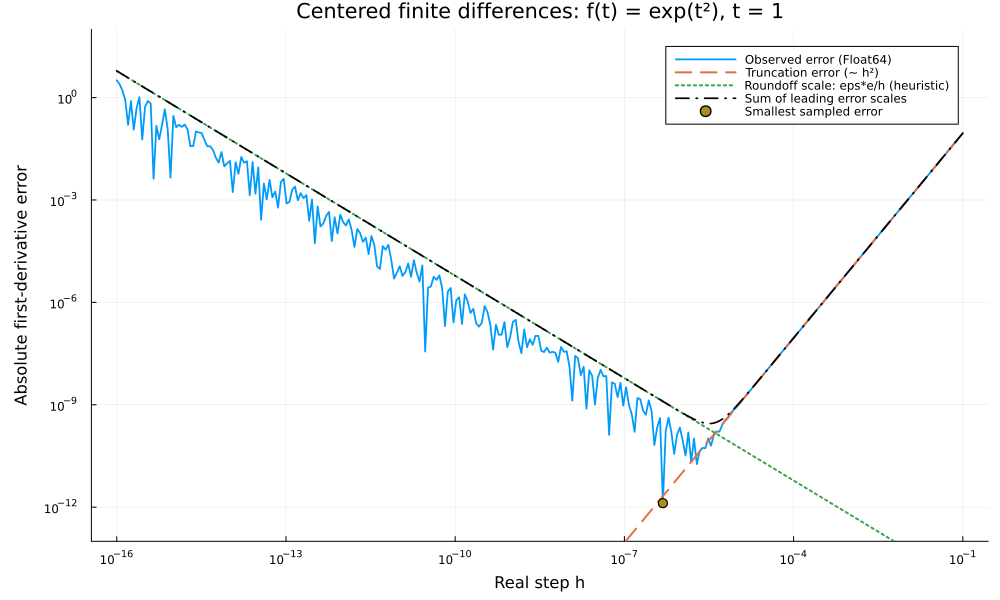
\includegraphics[width=0.95\linewidth]{../results/worked_example/fd_convergence.png}
\captionof{figure}{Centered finite-difference error for $f(t)=\exp(t^2)$ at
$t=1$. The observed error compares the Float64 derivative with a 256-bit
reference $2\mathrm e$. Truncation error is evaluated with the same centered
stencil in 256-bit arithmetic. The roundoff scale and summed error model
illustrate the competing trends; they are not bounds on the observed error.}
\label{fig:fd-example-convergence}
\end{center}
At large $h$, truncation dominates and the error decreases approximately as
$h^2$ when the step is reduced. At small $h$, cancellation and rounding dominate,
producing an irregular increase in error. The smallest observed error lies
between these regimes; its location depends on the function and arithmetic.
Figure~\ref{fig:ctse-example-convergence} contrasts this behavior with CTSE for
the same function and evaluation point.
The figure and raw error data can be regenerated from the repository root:
\begin{verbatim}
julia --project=. docs/fd_worked_example.jl
\end{verbatim}

\subsection{First derivatives with CTSE}
\label{sec:ctse}
Complex Taylor series expansion (CTSE), also called the complex-step method,
evaluates the response at a complex input $t+ih$, where $i^2=-1$ and $h>0$
is a small real step~\cite{martins2003}. If $F$ is analytic and real-valued on the real axis,
\[
 F(t+ih)=F(t)+ihF'(t)-\frac{h^2}{2}F''(t)
        -\frac{ih^3}{6}F'''(t)+O(h^4).
\]
Taking the imaginary part and dividing by $h$ gives
\begin{equation}
\label{eq:ctse-derivative}
 \boxed{F'(t)\approx\frac{\operatorname{Im}F(t+ih)}{h}},\qquad
 \frac{\operatorname{Im}F(t+ih)}{h}=F'(t)-\frac{h^2}{6}F'''(t)+O(h^4).
\end{equation}
The real part supplies $F(t)$ with an $O(h^2)$ error. Unlike a finite difference,
Equation~\eqref{eq:ctse-derivative} does not subtract nearly equal response values, allowing
a very small $h$. CTSE is a
numerical derivative approximation; OTI arithmetic, introduced in Section~\ref{sec:oti}, propagates
Taylor coefficients algebraically.

The evaluated function must admit an analytic extension near the real input.
Operations such as absolute values, conjugation, or premature removal of
imaginary components can invalidate the method. Standard CTSE provides the
first derivative in Equation~\eqref{eq:ctse-derivative}; one evaluation does not
separate the higher derivatives also present in its Taylor expansion. Other
complex-step extensions exist, but are outside the scope of this comparison.
\subsubsection{Worked example: \texorpdfstring{$f(t)=\exp(t^2)$}{f(t) = exp(t squared)}}
\label{sec:example-ctse}
Consider the composition $v=t^2$, $f=\exp(v)$ at $t_0=1$.
Sections~\ref{sec:example-oti} and~\ref{sec:example-cr} evaluate this same function
using OTI arithmetic and its CR representation. Direct differentiation supplies
reference values:
\begin{equation}
\label{eq:example-reference}
 f(1)=\mathrm e,\qquad f'(1)=2\mathrm e,\qquad f''(1)=6\mathrm e.
\end{equation}
Here $\mathrm e=\exp(1)$ is Euler's number. For CTSE, first seed the input as
$\widetilde t=1+ih$. Then evaluate the original two operations with complex
arithmetic, retaining the imaginary component at each step:
\begin{align*}
 \widetilde v&=(1+ih)^2=1-h^2+2ih,\\
 \widetilde f&=\exp(\widetilde v)
 =\exp(1-h^2)\bigl[\cos(2h)+i\sin(2h)\bigr].
\end{align*}
The real and imaginary parts therefore give
\begin{equation}
\label{eq:example-ctse}
 f(1)\approx\exp(1-h^2)\cos(2h),\qquad
 f'(1)\approx\exp(1-h^2)\frac{\sin(2h)}{h}.
\end{equation}
Expanding the extracted derivative in Equation~\eqref{eq:example-ctse} gives
\begin{equation}
\label{eq:example-ctse-error}
 \exp(1-h^2)\frac{\sin(2h)}{h}
 =2\mathrm e-\frac{10}{3}\mathrm e h^2+O(h^4).
\end{equation}
The leading term matches Equation~\eqref{eq:fd-example-error} in magnitude and
differs only in sign. This is not particular to the example: for any analytic
$F$, the centered difference carries $+h^2F'''(t)/6$ and the complex step
$-h^2F'''(t)/6$. The two methods therefore share the same truncation error, and
what separates them is the other error source. The centered difference forms
$F(t+h)-F(t-h)$, a subtraction of increasingly close values, so reducing $h$
eventually destroys accuracy through cancellation. The complex step takes an
imaginary part rather than a difference, so no such subtraction occurs and $h$
may be reduced far below the finite-difference optimum.

Equation~\eqref{eq:example-ctse-error} predicts second-order convergence as $h$
decreases, until numerical rounding dominates. Table~\ref{tab:ctse-example}
presents the computed function values and first derivatives for selected steps.
Figure~\ref{fig:ctse-example-convergence} shows the corresponding convergence
and the leading truncation-error magnitude $(10/3)\mathrm e h^2$.
The original operations are evaluated once per complex input; neither a
symbolic derivative nor a difference of nearby function values is needed.

\newpage
\paragraph{Numerical results for the worked example.}
The evaluations use Julia's ordinary \texttt{Float64} complex arithmetic.
The reference values are $f(1)=\mathrm e\approx2.718281828459$ and
$f'(1)=2\mathrm e\approx5.436563656918$. To distinguish rounding error from
truncation error, absolute errors are computed against a 256-bit evaluation of
$2\mathrm e$, using the full stored derivative rather than its printed digits.

\begin{center}
\captionof{table}{CTSE evaluations of $f(t)=\exp(t^2)$ at $t=1$. Function values
and derivatives are printed to twelve decimal places; errors use the full
stored values and a high-precision reference.}
\label{tab:ctse-example}
\smallskip
\begin{tabular}{rrrr}\toprule
Step $h$ & $\operatorname{Re}\widetilde f$ & $\operatorname{Im}\widetilde f/h$ & Absolute derivative error \\ \midrule
$1.000\times10^{-1}$ & 2.637588959484 & 5.346657516342 & $8.991\times10^{-2}$ \\
$1.000\times10^{-2}$ & 2.717466429984 & 5.435657633647 & $9.060\times10^{-4}$ \\
$1.000\times10^{-3}$ & 2.718273673622 & 5.436554595986 & $9.061\times10^{-6}$ \\
$1.000\times10^{-4}$ & 2.718281746911 & 5.436563566309 & $9.061\times10^{-8}$ \\
$1.000\times10^{-6}$ & 2.718281828451 & 5.436563656909 & $9.061\times10^{-12}$ \\
$1.000\times10^{-8}$ & 2.718281828459 & 5.436563656918 & $2.891\times10^{-16}$ \\
$1.000\times10^{-12}$ & 2.718281828459 & 5.436563656918 & $2.891\times10^{-16}$ \\
$1.000\times10^{-20}$ & 2.718281828459 & 5.436563656918 & $2.891\times10^{-16}$ \\
\bottomrule\end{tabular}

\end{center}

\begin{center}
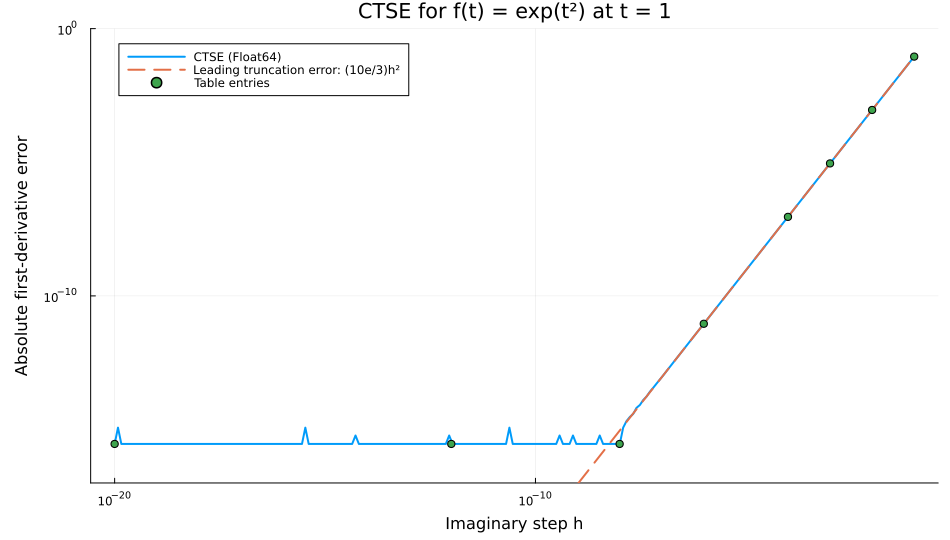
\includegraphics[width=0.92\linewidth]{../results/worked_example/ctse_convergence.png}
\captionof{figure}{CTSE first-derivative convergence for the worked example.
The dashed line is the leading truncation error from
Equation~\eqref{eq:example-ctse-error}; markers identify the steps in
Table~\ref{tab:ctse-example}.}
\label{fig:ctse-example-convergence}
\end{center}
Figure~\ref{fig:ctse-example-convergence} shows the error initially decreasing
in proportion to $h^2$. For sufficiently small steps, the error reaches a
floating-point rounding level and no longer decreases systematically.
Unlike real finite differences, reducing $h$ further does not introduce
subtractive cancellation in the derivative extraction for this example.
The table, figure, and raw CSV data can be regenerated from the repository root:
\begin{verbatim}
julia --project=. docs/ctse_worked_example.jl
\end{verbatim}

\newpage
\subsection{OTI arithmetic and Taylor coefficients}
\label{sec:oti}
For one variable and truncation order $p$, consider two order-truncated imaginary
(OTI) numbers~\cite{aristizabal2020}:
\begin{equation}
\label{eq:oti-factors}
 a=\sum_{j=0}^{p}a_j\varepsilon^j,\qquad
 b=\sum_{j=0}^{p}b_j\varepsilon^j,\qquad
 a_j,b_j\in\mathbb R,\quad\varepsilon^{p+1}=0.
\end{equation}
The symbol $\varepsilon$ is \emph{nilpotent}: sufficiently high powers vanish.
It is neither a small floating-point number nor the usual complex unit
$i$ with $i^2=-1$.

At $p=1$, Equation~\eqref{eq:oti-factors} reduces to the \emph{dual numbers}
$a_0+a_1\varepsilon$ with $\varepsilon^2=0$, which carry a value and one
derivative through a forward-mode evaluation. OTI numbers extend that same
construction to order $p$, carrying $p$ derivatives at once.

The prescribed square is also what separates this from Section~\ref{sec:ctse}.
Under the complex step, $i^2=-1$ folds the third-order Taylor term back into the
imaginary part, which is the origin of the $O(h^2)$ truncation error in
Equation~\eqref{eq:ctse-derivative}. Nilpotency annihilates that term instead,
so the retained coefficients are exact in the algebra rather than approximations
improved by shrinking a step. The name retains \emph{imaginary} because the
construction parallels $\mathbb C$, adjoining to the reals a new unit with a
prescribed square, and because extracting a coefficient plays the role of taking
an imaginary part, as the notation $\operatorname{Im}_{\varepsilon^k}$ in
Equation~\eqref{eq:oti-extraction} reflects.

Addition combines coefficients of the same power:
\begin{equation}
\label{eq:oti-addition}
 a+b=\sum_{j=0}^{p}(a_j+b_j)\varepsilon^j.
\end{equation}
At order two, Equation~\eqref{eq:oti-addition} becomes
\[
 a+b=(a_0+b_0)+(a_1+b_1)\varepsilon+(a_2+b_2)\varepsilon^2.
\]
Multiplication collects terms
of equal degree and discards terms above order $p$:
\[
 ab=\sum_{k=0}^{p}\left(\sum_{j=0}^{k}a_jb_{k-j}\right)\varepsilon^k.
\]
For example, at order two, $a=a_0+a_1\varepsilon+a_2\varepsilon^2$ and
$b=b_0+b_1\varepsilon+b_2\varepsilon^2$ give
\[
 ab=a_0b_0+(a_0b_1+a_1b_0)\varepsilon
 +(a_0b_2+a_1b_1+a_2b_0)\varepsilon^2.
\]
The coefficient $a_0b_1+a_1b_0$ reproduces the first-derivative product rule
when the inputs carry Taylor coefficients.

An OTI scalar type can support \emph{operator overloading}: operations such as
addition and multiplication are defined to combine coefficients according
to these rules. Elementary functions such as $\exp$ and $\sin$ can likewise be
overloaded using their Taylor expansions. For
$a=a_0+\sum_{r=1}^{p}a_r\varepsilon^r$, the expansion about its real part $a_0$
is evaluated at the full OTI input as
\begin{equation}
\label{eq:oti-function}
 g\!\left(a_0+\sum_{r=1}^{p}a_r\varepsilon^r\right)
 =\sum_{j=0}^{p}\frac{g^{(j)}(a_0)}{j!}
     \left(\sum_{r=1}^{p}a_r\varepsilon^r\right)^j.
\end{equation}
Powers above $p$ vanish because the displacement has zero constant coefficient
and $\varepsilon^{p+1}=0$. For example, at order two,
\[
 \exp(a_0+a_1\varepsilon+a_2\varepsilon^2)
 =\exp(a_0)\left[1+(a_1\varepsilon+a_2\varepsilon^2)
                  +\frac{(a_1\varepsilon+a_2\varepsilon^2)^2}{2}\right].
\]
A calculation composed of supported operations then propagates coefficients
through the same sequence of function evaluations. Section~\ref{sec:cr}
provides an equivalent real matrix representation; the implementation in
Section~\ref{sec:oti-thermal} uses that representation rather than defining
an overloaded OTI scalar type.

Seeding the input as $t+\varepsilon$ gives, for an analytic function,
\begin{equation}
\label{eq:oti-taylor}
 F(t+\varepsilon)=F(t)+F'(t)\varepsilon+
 \frac{F''(t)}{2!}\varepsilon^2+\cdots+
 \frac{F^{(p)}(t)}{p!}\varepsilon^p.
\end{equation}
Define $\operatorname{Im}_{\varepsilon^k}(a):=a_k$ to mean extraction of the
coefficient of $\varepsilon^k$; this is not the ordinary complex imaginary-part
operator. Equation~\eqref{eq:oti-taylor} therefore yields the unscaled derivative
\begin{equation}
\label{eq:oti-extraction}
 \boxed{F^{(k)}(t)=k!\,\operatorname{Im}_{\varepsilon^k}
       \bigl(F(t+\varepsilon)\bigr)},\qquad 1\leq k\leq p.
\end{equation}
The constant coefficient is $F(t)$. The unit seed in $t+\varepsilon$ fixes the
scaling in Equation~\eqref{eq:oti-extraction}; no numerical perturbation step is
required. For example, $(t+\varepsilon)^2=t^2+2t\varepsilon+\varepsilon^2$,
so the second derivative is $2!\times1=2$.
Truncation does not approximate the retained Taylor coefficients in exact
arithmetic; numerical computations still incur floating-point error.

\subsubsection{Worked example: \texorpdfstring{$f(t)=\exp(t^2)$}{f(t) = exp(t squared)}}
\label{sec:example-oti}
Use the function and evaluation point of Section~\ref{sec:example-ctse}, now
with truncation order $p=2$. Seed $\widehat t=1+\varepsilon$ and impose $\varepsilon^3=0$. The square is obtained by
multiplying two OTI numbers $a=b=1+\varepsilon$:
\[
 \widehat v=\widehat t\,\widehat t=1+2\varepsilon+\varepsilon^2.
\]
The coefficients of $\widehat v$ are therefore $1$, $2$, and $1$. The next operation
is $g(v)=\exp(v)$. Its input is the OTI number $\widehat v$, which is decomposed
into a real part and a perturbation expressed in powers of $\varepsilon$:
\begin{equation}
\label{eq:oti-example-real-part}
 \widehat v=v_0+2\varepsilon+\varepsilon^2,\qquad v_0=1.
\end{equation}
The Taylor series expansion (TSE) is taken \emph{about the real part $v_0$}.
Before substituting the OTI input, write the expansion at a general argument $s$:
\begin{equation}
\label{eq:oti-example-tse}
 g(s)=g(v_0)+g'(v_0)(s-v_0)
       +\frac{g''(v_0)}{2!}(s-v_0)^2
       +\sum_{j=3}^{\infty}\frac{g^{(j)}(v_0)}{j!}(s-v_0)^j.
\end{equation}
Now evaluate Equation~\eqref{eq:oti-example-tse} at the full OTI argument
$s=\widehat v=v_0+2\varepsilon+\varepsilon^2$. The displacement from the
expansion point is $(v_0+2\varepsilon+\varepsilon^2)-v_0=2\varepsilon+\varepsilon^2$,
giving
\begin{align}
 g(v_0+2\varepsilon+\varepsilon^2)
 &=g(v_0)+g'(v_0)\bigl[(v_0+2\varepsilon+\varepsilon^2)-v_0\bigr]\notag\\
 &\quad+\frac{g''(v_0)}{2!}\bigl[(v_0+2\varepsilon+\varepsilon^2)-v_0\bigr]^2\notag\\
 &=g(v_0)+g'(v_0)(2\varepsilon+\varepsilon^2)
   +\frac{g''(v_0)}{2!}(2\varepsilon+\varepsilon^2)^2.
 \label{eq:oti-example-substitution}
\end{align}
Terms of degree three and higher vanish because
$(2\varepsilon+\varepsilon^2)^3=0$ in the order-two
algebra. Equation~\eqref{eq:oti-example-substitution} is therefore exact in that
algebra, rather than an approximation obtained by assuming a small real
perturbation. The function and its elementary derivatives are evaluated at the
real scalar $v_0$; the powers of the displacement use OTI arithmetic.

For the exponential, $g(1)=g'(1)=g''(1)=\mathrm e$. Substituting these real
values and the perturbation from Equation~\eqref{eq:oti-example-real-part} gives
\[
 \exp(1+2\varepsilon+\varepsilon^2)=\mathrm e+\mathrm e(2\varepsilon+\varepsilon^2)
       +\frac{\mathrm e}{2!}(2\varepsilon+\varepsilon^2)^2.
\]
The remaining multiplication is truncated according to $\varepsilon^3=0$:
\[
 (2\varepsilon+\varepsilon^2)^2
 =4\varepsilon^2+4\varepsilon^3+\varepsilon^4=4\varepsilon^2.
\]
Collecting equal powers of $\varepsilon$ yields the output of the overloaded
exponential:
\begin{equation}
\label{eq:example-oti}
 \widehat f=\mathrm e+2\mathrm e\,\varepsilon
       +\mathrm e\,\varepsilon^2+2\mathrm e\,\varepsilon^2
       =\mathrm e+2\mathrm e\,\varepsilon+3\mathrm e\,\varepsilon^2.
\end{equation}
The exponential's overload uses its known derivatives at the real part; it does
not require a manually derived formula for the derivative of the full
composition $f(t)=\exp(t^2)$.
Its coefficients are $\mathrm e$, $2\mathrm e$, and $3\mathrm e$.
Applying Equation~\eqref{eq:oti-extraction} gives
\[
 f(1)=\mathrm e,\qquad
 f'(1)=1!\,(2\mathrm e)=2\mathrm e,\qquad
 f''(1)=2!\,(3\mathrm e)=6\mathrm e.
\]
The second-order coefficient is $3\mathrm e$, whereas the second derivative is
$6\mathrm e$. These results match Equation~\eqref{eq:example-reference} exactly
in the truncated algebra, without choosing a numerical step size.
The evaluation trace still consists of a multiplication followed by an
exponential; the definitions of those operations propagate the coefficients.
Section~\ref{sec:example-cr} performs this same calculation using real matrices.

\newpage
\subsection{Cauchy--Riemann matrix representation}
\label{sec:cr}
Let $N$ be the $(p+1)\times(p+1)$ matrix with ones immediately below the diagonal
and zeros elsewhere. Since $N^{p+1}=0$, the OTI number defined in Section~\ref{sec:oti} has the representation
$C(a)=\sum_{j=0}^p a_jN^j$. At order two,
\[
 N=\begin{bmatrix}0&0&0\\1&0&0\\0&1&0\end{bmatrix},\qquad
 C(a)=\begin{bmatrix}a_0&0&0\\a_1&a_0&0\\a_2&a_1&a_0\end{bmatrix}.
\]
Multiplying $C(a)$ by the coefficient vector $[b_0,b_1,b_2]^T$ produces the
coefficients of $ab$. Consequently,
\[
 C(a+b)=C(a)+C(b),\qquad C(ab)=C(a)C(b).
\]
This is the generalized Cauchy--Riemann representation used here: a real matrix
implements OTI multiplication. The convention adopted here uses lower triangular matrices
and coefficients ordered by increasing degree. An upper triangular convention
would require corresponding changes in extraction.

For a square matrix whose entries are OTI numbers, collect the coefficients
of equal degree into ordinary real matrices:
\begin{equation}
\label{eq:matrix-coefficients}
 M=M_0+M_1\varepsilon+M_2\varepsilon^2,
 \qquad M_j\in\mathbb R^{m\times m}.
\end{equation}
Specifically, if entry $(r,s)$ is
$M_{rs}=m_{rs,0}+m_{rs,1}\varepsilon+m_{rs,2}\varepsilon^2$, then
$(M_j)_{rs}=m_{rs,j}$. Thus $M_j$ contains the order-$j$ coefficient of every
entry of $M$; its entries are real scalars, not OTI numbers.
The corresponding representation is a \emph{block matrix of coefficient matrices}:
\begin{equation}
\label{eq:matrix-cr}
 \mathcal C(M)=\begin{bmatrix}M_0&0&0\\M_1&M_0&0\\M_2&M_1&M_0\end{bmatrix}
 \in\mathbb R^{3m\times3m}.
\end{equation}
Every displayed block in Equation~\eqref{eq:matrix-cr}, including each zero block,
has size $m\times m$. The complete block array is an ordinary real
$3m\times3m$ matrix, suitable for real matrix operations. At truncation order $p$, the assembled matrix has size
$(p+1)m\times(p+1)m$.

It preserves matrix products, including their order. Because the exponential is
defined by a convergent series of sums and products, it also preserves the
matrix exponential. This lets a real-valued numerical routine evaluate the
OTI exponential without requiring a custom scalar type.


\newpage
\subsubsection{Worked example: \texorpdfstring{$f(t)=\exp(t^2)$}{f(t) = exp(t squared)}}
\label{sec:example-cr}
Represent the order-two seed $\widehat t=1+\varepsilon$ from
Section~\ref{sec:example-oti} by the ordinary real matrix
\[
 T=C(\widehat t)=I_3+N=
 \begin{bmatrix}1&0&0\\1&1&0\\0&1&1\end{bmatrix}.
\]
The same evaluation trace becomes a matrix multiplication followed by a matrix
exponential. The first operation gives
\[
 V=T^2=I_3+2N+N^2=
 \begin{bmatrix}1&0&0\\2&1&0\\1&2&1\end{bmatrix}.
\]
Thus $V=C(1+2\varepsilon+\varepsilon^2)$: its first column contains exactly
the intermediate coefficients from Section~\ref{sec:example-oti}.
For the second operation, write $V=I_3+K$ with $K=2N+N^2$.
Since $K^2=4N^2$ and $K^3=0$, the matrix exponential reduces to
\begin{equation}
\label{eq:example-cr}
 W=\exp(V)=\mathrm e\left(I_3+K+\frac{K^2}{2}\right)
 =\mathrm e\begin{bmatrix}1&0&0\\2&1&0\\3&2&1\end{bmatrix}.
\end{equation}
The first column of $W$, equivalently $W[1,0,0]^T$, is
$[\mathrm e,2\mathrm e,3\mathrm e]^T$. It contains the Taylor coefficients,
so multiplying the third entry by $2!$ yields the second derivative:
\[
 f(1)\approx2.718281828459,\qquad
 f'(1)\approx5.436563656918,\qquad
 f''(1)\approx16.309690970754.
\]
These are the same results as Equation~\eqref{eq:example-oti}. No OTI scalar type
is required: an ordinary real matrix multiplication computes $T^2$, and a real
matrix-exponential routine computes $\exp(V)$. These are matrix operations,
not entrywise squaring or exponentiation. The matrix representation changes
how the coefficients are stored and propagated; the factorial extraction rule
remains the same as in Section~\ref{sec:oti}.

\clearpage
\section{Implementation}
\label{sec:implementation}
\subsection{Original response calculation}
\label{sec:baseline}
The repository example evaluates a vector response $F(\Delta t)$ containing ten
final voxel temperatures. The differentiation parameter is the duration
$\Delta t$, nominally 50 s; the arrays $A,B,e,x_k,u$ remain fixed. The original
\texttt{MatrixExponentialTest.jl} is retained without modification. Separate
entry points, \texttt{CTSEExample.jl} and \texttt{CRExample.jl}, call reusable
functions implementing the methods of Section~\ref{sec:background}.

The calculation already uses an augmented matrix exponential:
\begin{equation}
\label{eq:baseline-response}
 H=\begin{bmatrix}A&B&I_n\\0&0&0\\0&0&0\end{bmatrix},\qquad
 z_0=\begin{bmatrix}x_k\\u\\e\end{bmatrix},\qquad
 F(t)=P_x\exp(tH)z_0,\quad P_x=[I_n\;0\;0].
\end{equation}
Here $P_x$ selects the first $n$ entries. The top block row of $\exp(tH)$ supplies
$A_d$, $B_d$, and the integrated forcing $e_d$, giving $F(t)=A_dx_k+B_du+e_d$.
No additional physical model is required to apply the differentiation methods.
The shared \texttt{response} function in \texttt{src/OTISensitivity.jl}
encapsulates this calculation as shown in Listing~\ref{lst:response}.
\begin{lstlisting}[caption={Reusable response evaluation.},label={lst:response}]
function response(A, B, e, x, u, dt)
    Ad, Bd, ed = discretize_linear_dynamics(A, B, e, dt)
    return Ad*x + Bd*u + ed
end
\end{lstlisting}
The original final update adds $e$ rather than $e_d$. Its example has $e=0$, so
this distinction does not change its result. The shared routine uses $e_d$ and
is tested with nonzero forcing. This correction and the extraction of reusable
functions are supporting changes, independent of either differentiation method.

\subsection{CTSE: complex input and derivative extraction}
\label{sec:ctse-code}
\label{sec:ctse-thermal}
Applying Section~\ref{sec:ctse} requires replacing $t_0$ by $t_0+ih$ in
Equation~\eqref{eq:baseline-response}. Consequently,
\begin{align}
 \widetilde M&=(t_0+ih)H=t_0H+ihH,\label{eq:ctse-matrix}\\
 \widetilde F&=P_x\exp(\widetilde M)z_0.\label{eq:ctse-response}
\end{align}
Only the duration is perturbed. The matrix $H$ and vector $z_0$ retain their
original real values. The scaled matrix becomes complex, while its size remains
$21\times21$. Since $H$ is constant,
\[
 \widetilde F=F(t_0)+ih\,P_xH\exp(t_0H)z_0+O(h^2),
\]
so the coefficient of $ih$ is the requested derivative $F'(t_0)$.

The original routine forms a real matrix $H$ and scales it in place
(Listing~\ref{lst:original-exponential}). A complex timestep cannot be stored in
that real array. The shared routine therefore allocates the scaled matrix out of
place (Listing~\ref{lst:complex-exponential}); its timestep argument accepts
\texttt{dt::Number}, including complex values.
\begin{lstlisting}[caption={Matrix scaling and exponential in the original script.},label={lst:original-exponential}]
H .*= dt
G = exponential!(H)
\end{lstlisting}
\begin{lstlisting}[caption={Replacement in the shared discretization routine.},label={lst:complex-exponential}]
G = exponential!(augmented_dynamics(A, B) * dt)
\end{lstlisting}

\newpage
\texttt{ctse\_response} in \texttt{src/SensitivityComparison.jl} then passes the
complex timestep through the response routine and extracts the result as shown
in Listing~\ref{lst:ctse}. The example uses $h=10^{-20}$ s.
\begin{lstlisting}[caption={CTSE evaluation and extraction; input validation is omitted from this excerpt.},label={lst:ctse}]
z = response(A, B, e, x, u, complex(dt, h))
return (; value=real.(z), derivative=imag.(z)/h)
\end{lstlisting}
Here \texttt{z} is the complex response $\widetilde F$, not the augmented vector
$z_0$. The matrix-exponential routine, block extraction, and response multiplication
follow the same calculation as the real evaluation. Complex components are
preserved until the final real and imaginary extraction in
Equation~\eqref{eq:ctse-derivative}; no sensitivity equation is added.
\texttt{CTSEExample.jl} saves these values and first derivatives to
\texttt{results/ctse.csv}. Figure~\ref{fig:derivatives}, upper-left panel, compares
its first derivatives with the other methods; Figure~\ref{fig:step-convergence},
upper-left panel, assesses the imaginary step size.

\subsection{OTI--CR: real block assembly and coefficient extraction}
\label{sec:oti-thermal}
For the method of Sections~\ref{sec:oti} and~\ref{sec:cr}, the seeded duration is
$t_0+\varepsilon$. At second order, the OTI matrix $M=(t_0+\varepsilon)H$ has
coefficient matrices $M_0=t_0H$, $M_1=H$, and $M_2=0$. Substitution into
Equation~\eqref{eq:matrix-cr} gives
\begin{equation}
\label{eq:lifted-matrix}
 \mathcal H=C(t_0+\varepsilon)\otimes H
 =\begin{bmatrix}t_0H&0&0\\H&t_0H&0\\0&H&t_0H\end{bmatrix}.
\end{equation}
The Kronecker product $\otimes$ replaces each scalar entry by that scalar times
$H$. Every block is $21\times21$; Julia assembles a single real $63\times63$
matrix. At order $p$, its dimension is $21(p+1)$.

Instead of passing $t_0H$ to the exponential, \texttt{oti\_response} in
\texttt{src/OTISensitivity.jl} passes the block representation, as shown in
Listing~\ref{lst:cr-assembly}. The helper \texttt{oti\_matrix(seed)} constructs
$C(t_0+\varepsilon)$ from the coefficients $[t_0,1,0,\ldots,0]$.
\begin{lstlisting}[caption={OTI seed and real block exponential.},label={lst:cr-assembly}]
H = augmented_dynamics(A, B)
seed = zeros(promote_type(Float64, typeof(dt)), order+1)
seed[1] = dt
order > 0 && (seed[2] = 1)
G = exponential!(kron(oti_matrix(seed), H))
\end{lstlisting}
Write $G_0(t)=\exp(tH)$. The second-order lifted exponential satisfies
\begin{equation}
\label{eq:cr-exponential}
 \exp(\mathcal H)=
 \begin{bmatrix}G_0&0&0\\G_0'&G_0&0\\G_0''/2!&G_0'&G_0\end{bmatrix}.
\end{equation}
The first block column, multiplied by $z_0$, contains the response coefficients.
The top $n$ entries of block $j$ yield $F^{(j)}(t_0)/j!$.

\newpage
Listing~\ref{lst:cr-extraction} shows the corresponding extraction and factorial
scaling. Here \texttt{m} is the augmented dimension, \texttt{n} is the number of
response entries, and \texttt{G} is the lifted exponential of
Equation~\eqref{eq:cr-exponential}.
\begin{lstlisting}[caption={Extraction of OTI coefficients and conversion to derivatives.},label={lst:cr-extraction}]
m = size(H, 1)
z = vcat(x, u, e)
coefficients = hcat([G[j*m+1:j*m+n, 1:m] * z for j in 0:order]...)
derivatives = copy(coefficients)
factor = one(eltype(derivatives))
for j in 1:order
    factor *= j
    derivatives[:, j+1] .*= factor
end
\end{lstlisting}
Column one contains the nominal value. Column $j+1$ of \texttt{coefficients}
contains the order-$j$ Taylor coefficient; the same column of \texttt{derivatives}
contains the actual derivative. \texttt{CRExample.jl} saves orders zero through
four to \texttt{results/cr.csv}. The scalar type remains real; the changes are
the larger matrix passed to the solver and the extraction of its coefficient
blocks. Dense storage grows quadratically and typical dense exponential work
cubically with the enlarged dimension. This implementation is a baseline for
method comparisons rather than an optimized solver.

\subsection{Comparison and verification code}
\label{sec:verification}
\texttt{CompareSensitivities.jl} runs the unchanged original in an isolated Julia
module, runs the implementations in Section~\ref{sec:implementation}, and writes comparison CSV files and plots.
The original supplies a function value only; it has no derivative implementation.
The ``FD baseline'' function value is the unperturbed real response, not a derivative.

For derivative order $j=1,\ldots,4$, finite differences (FD) use seven real
response evaluations:
\begin{equation}
\label{eq:finite-difference}
 D_j(h)=h^{-j}\sum_{k=-3}^{3}w_k^{(j)}F(t+kh),\qquad
 \sum_{k=-3}^{3}w_k^{(j)}k^q=
 \begin{cases}j!,&q=j,\\0,&0\leq q\leq6,\ q\ne j.\end{cases}
\end{equation}
The moment conditions in Equation~\eqref{eq:finite-difference} make the formula exact for polynomials through degree six.
The weights are computed in exact rational arithmetic, then converted to floating
point for use with response values. Symmetry gives truncation error $O(h^6)$
for orders one and two, and $O(h^4)$ for orders three and four.
Small $h$ increases cancellation and roundoff, roughly as
$\epsilon_{\rm mach}/h^j$. The selected step is
$h_j=\max(|t|,1)\epsilon_{\rm mach}^{1/(j+a_j)}$ in the code's seconds convention,
where $a_j$ is six or four respectively. At $t=50$ s these steps are approximately
$0.290$, $0.552$, $0.290$, and $0.552$ s. This is a heuristic balance, not a
universal optimal step. Figure~\ref{fig:step-convergence} presents a sweep of $h$ to assess its effect.

An independent derivative reference follows by differentiating the augmented
response $F(t)=P_x\exp(tH)z_0$ defined in Section~\ref{sec:baseline}:
\begin{equation}
\label{eq:analytical}
 F'=AF+Bu+e,\qquad F^{(j)}=AF^{(j-1)}\quad(j\geq2).
\end{equation}
The reference value $F$ is computed by diagonalizing the symmetric $A$ and
integrating each scalar mode. The forcing integral is
$(\exp(\lambda t)-1)/\lambda$, with limit $t$ at $\lambda=0$.
This handles the insulated model's zero mode without inverting its singular $A$.
Errors are measured against Equation~\eqref{eq:analytical} and the modal reference
value. Absolute errors have units K/s$^j$; relative errors are
$\|y-y_{\rm ref}\|_\infty/\|y_{\rm ref}\|_\infty$ over all ten voxels, avoiding
division by an individual near-zero derivative. The comparison also directly
checks CTSE against OTI--CR and FD against OTI--CR.


The scripts can be executed from the repository root using:
\begin{verbatim}
julia --project=. CTSEExample.jl
julia --project=. CRExample.jl
julia --project=. CompareSensitivities.jl
julia --project=. test/runtests.jl
\end{verbatim}
The comparison script writes per-voxel values and derivatives, error summaries,
and step sweeps to CSV files in \texttt{results/}. The figures and table in
Section~\ref{sec:results} are generated from these evaluations.
\newpage
\section{Results}
\label{sec:results}
\subsection{Function values and derivative agreement}
\label{sec:agreement}
The implementations in Sections~\ref{sec:ctse-code} and~\ref{sec:oti-thermal} are evaluated at
$\Delta t=50$ s using the verification procedure in Section~\ref{sec:verification}.
Table~\ref{tab:agreement} reports errors against the independent analytical
reference. The CTSE and OTI--CR first derivatives have relative errors of
approximately $2.54\times10^{-14}$ and $1.64\times10^{-14}$, respectively.
FD agrees through fourth order, with its relative error increasing from
$1.39\times10^{-11}$ at first order to $2.10\times10^{-5}$ at fourth order.
This reduced accuracy is consistent with the cancellation described in
Section~\ref{sec:verification}; FD provides corroborating evidence rather than
an exact reference.

\par\medskip
\noindent\begin{minipage}{\linewidth}
\captionof{table}{Errors at $\Delta t=50$ s relative to the independent analytical
reference. Order zero denotes the function value. Absolute errors have units
K/s$^j$ for derivative order $j$; relative infinity errors are dimensionless.}
\label{tab:agreement}
\begin{center}\begin{tabular}{lrrr}\toprule
Method & Order & Max. absolute error & Relative infinity error \\ \midrule
Original & 0 & 1.78e-11 & 3.03e-14 \\
CTSE & 0 & 1.38e-11 & 2.34e-14 \\
CTSE & 1 & 9.81e-14 & 2.54e-14 \\
OTI-CR & 0 & 1.78e-11 & 3.03e-14 \\
OTI-CR & 1 & 6.35e-14 & 1.64e-14 \\
OTI-CR & 2 & 6.80e-15 & 1.16e-13 \\
OTI-CR & 3 & 9.70e-16 & 3.72e-13 \\
OTI-CR & 4 & 1.38e-16 & 8.70e-13 \\
FD & 0 & 1.78e-11 & 3.03e-14 \\
FD & 1 & 5.37e-11 & 1.39e-11 \\
FD & 2 & 2.45e-10 & 4.17e-09 \\
FD & 3 & 1.51e-09 & 5.81e-07 \\
FD & 4 & 3.33e-09 & 2.10e-05 \\
\bottomrule\end{tabular}\end{center}

\end{minipage}
\par\medskip

Figure~\ref{fig:values} shows agreement of the nominal temperatures across the
original script, CTSE, OTI--CR, and the real response used as the FD baseline.
Figure~\ref{fig:derivatives} compares the corresponding voxel sensitivities;
CTSE appears only in the first-order panel.
\begin{center}
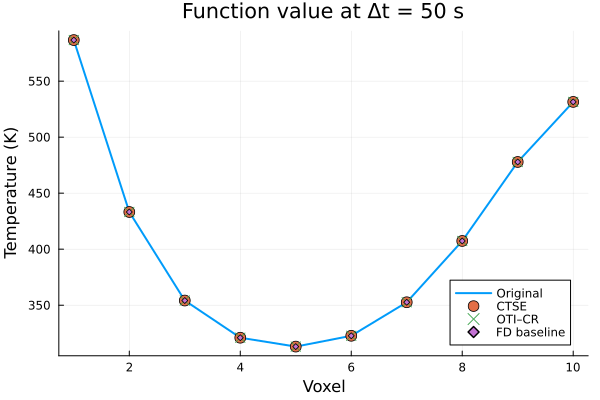
\includegraphics[width=0.68\linewidth]{../results/function_values.png}
\captionof{figure}{Nominal voxel temperatures at $\Delta t=50$ s. CTSE and OTI--CR
agree with the unchanged original script and the unperturbed real FD baseline.}
\label{fig:values}
\end{center}
All 246 test assertions pass. The tests cover scalar derivatives, OTI algebra,
zero duration, nonzero forcing, CTSE steps from $10^{-8}$ to $10^{-30}$ s,
and FD polynomial exactness.

\newpage
\subsection{Derivative profiles and step-size dependence}
\label{sec:step-results}

\begin{center}
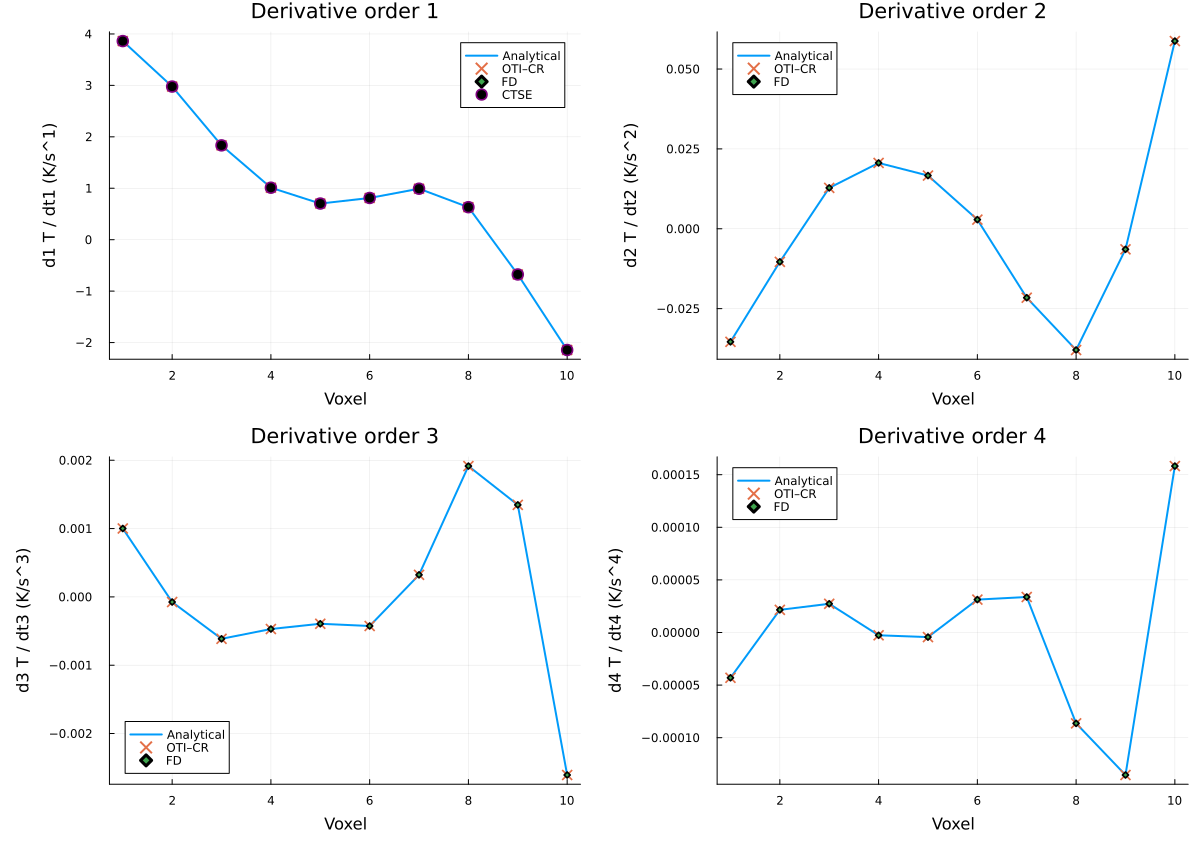
\includegraphics[width=0.62\linewidth]{../results/derivatives.png}
\captionof{figure}{Voxel temperature derivatives at $\Delta t=50$ s. The
upper-left panel compares CTSE, OTI--CR, FD, and the analytical first derivative.
CTSE is omitted from orders two through four.}
\label{fig:derivatives}
\end{center}
\begin{center}
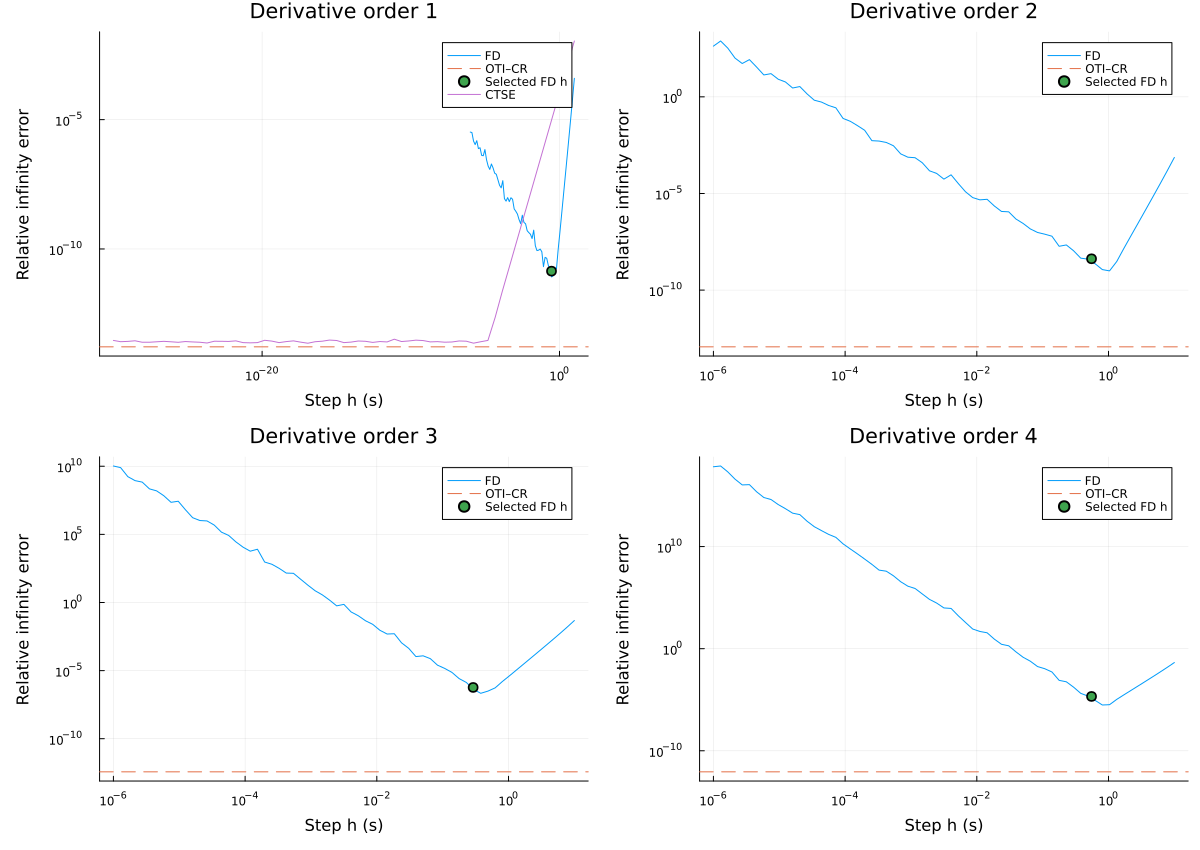
\includegraphics[width=0.62\linewidth]{../results/step_convergence.png}
\captionof{figure}{Relative derivative errors versus step size. The upper-left
panel compares the CTSE imaginary-step sweep with real finite differences (FD).
OTI--CR has no step parameter and is shown as a horizontal reference. Higher-order
panels show FD and OTI--CR only.}
\label{fig:step-convergence}
\end{center}
Figure~\ref{fig:step-convergence} shows FD accuracy deteriorating for both small
and large steps. CTSE maintains first-derivative accuracy for very small imaginary
steps in this example. OTI--CR has no step parameter and provides a horizontal
error reference. Errors in Figure~\ref{fig:step-convergence} are floored at machine
epsilon only for logarithmic display; the CSV files retain the raw errors.

\clearpage
\begingroup
\small
\begin{thebibliography}{9}
\bibitem{ADinML}
A. G. Baydin, B. A. Pearlmutter, A. A. Radul, and J. M. Siskind (2018).
\href{https://jmlr.org/papers/v18/17-468.html}{Automatic Differentiation in Machine Learning: a Survey}.
\emph{Journal of Machine Learning Research}, 18(153), 1--43.
\bibitem{AD-App}
C. H. Bischof, H. M. B\"ucker, P. Hovland, U. Naumann, and J. Utke (eds., 2008).
\href{https://link.springer.com/book/10.1007/978-3-540-68942-3}{Advances in Automatic Differentiation}.
Springer.
\bibitem{eval_deriv_ad}
A. Griewank and A. Walther (2008).
\href{https://epubs.siam.org/doi/book/10.1137/1.9780898717761}{Evaluating Derivatives: Principles and Techniques of Algorithmic Differentiation}.
Second edition, SIAM.
\bibitem{martins-guide}
MDO Lab. \href{https://mdolab.engin.umich.edu/wiki/guide-complex-step-derivative-approximation}{A Guide to the Complex-Step Derivative Approximation}.
\bibitem{martins2003}
J. R. R. A. Martins, P. Sturdza, and J. J. Alonso (2003).
\href{https://mdolab.engin.umich.edu/bibliography/Martins2003a}{The Complex-Step Derivative Approximation}.
\bibitem{aristizabal2020}
M. Aristizabal Cano (2020).
\href{https://repository.eafit.edu.co/bitstreams/cc604c41-15b6-4a47-a076-0aec419e6391/download}{Order truncated imaginary algebra for computation of multivariable high-order derivatives in finite element analysis}.
\end{thebibliography}
\endgroup
\end{document}
